\documentclass[12pt]{article}
\usepackage[spanish, english, es-tabla]{babel}
\usepackage[utf8]{inputenc}
\usepackage[left = 2cm, right = 2cm, bottom = 2cm, top = 3cm]{geometry}
\usepackage{amsmath, amssymb}
\usepackage{graphicx}
\usepackage [hidelinks]{hyperref}
\usepackage[usenames,dvipsnames]{xcolor}

%%PACKAGES FOR COVER PAGE%%

\usepackage{tikz}
\usetikzlibrary{calc}
\usepackage{anyfontsize}
\usepackage{sectsty}

%%SETUP FOR PDF PROPERTIES%%
\hypersetup{
	pdftitle={Hackathon AllWize: WizeTher},
	pdfsubject={Telecomunicaciones},
	pdfauthor={Enrique Fernández Sánchez, Lucía Francoso Fernández},
	pdfkeywords={Wize, AllWize, WizeTher, calidad aire, openData}
} 

%% SETUP FOR THE LINKS%%
\hypersetup{
	colorlinks,
    linkcolor=black,
	citecolor={blue!50!black},
	urlcolor=cyan
}

\begin{document}
	\selectlanguage{spanish}
	
%% COVER PAGE %%

\pagestyle{empty}

\begin{tikzpicture}[overlay,remember picture]
	
	% Background color
	\fill[
	black!2]
	(current page.south west) rectangle (current page.north east);
	
	% Rectangles
	\shade[
	left color=Dandelion, 
	right color=Dandelion!40,
	transform canvas ={rotate around ={45:($(current page.north west)+(0,-6)$)}}] 
	($(current page.north west)+(0,-6)$) rectangle ++(9,1.5);
	
	\shade[
	left color=lightgray,
	right color=lightgray!50,
	rounded corners=0.75cm,
	transform canvas ={rotate around ={45:($(current page.north west)+(.5,-10)$)}}]
	($(current page.north west)+(0.5,-10)$) rectangle ++(15,1.5);
	
	\shade[
	left color=lightgray,
	rounded corners=0.3cm,
	transform canvas ={rotate around ={45:($(current page.north west)+(.5,-10)$)}}] ($(current page.north west)+(1.5,-9.55)$) rectangle ++(7,.6);
	
	\shade[
	left color=orange!80,
	right color=orange!60,
	rounded corners=0.4cm,
	transform canvas ={rotate around ={45:($(current page.north)+(-1.5,-3)$)}}]
	($(current page.north)+(-1.5,-3)$) rectangle ++(9,0.8);
	
	\shade[
	left color=red!80,
	right color=red!80,
	rounded corners=0.9cm,
	transform canvas ={rotate around ={45:($(current page.north)+(-3,-8)$)}}] ($(current page.north)+(-3,-8)$) rectangle ++(15,1.8);
	
	\shade[
	left color=orange,
	right color=Dandelion,
	rounded corners=0.9cm,
	transform canvas ={rotate around ={45:($(current page.north west)+(4,-15.5)$)}}]
	($(current page.north west)+(4,-15.5)$) rectangle ++(30,1.8);
	
	\shade[
	left color=RoyalBlue,
	right color=Emerald,
	rounded corners=0.75cm,
	transform canvas ={rotate around ={45:($(current page.north west)+(13,-10)$)}}]
	($(current page.north west)+(13,-10)$) rectangle ++(15,1.5);
	
	\shade[
	left color=lightgray,
	rounded corners=0.3cm,
	transform canvas ={rotate around ={45:($(current page.north west)+(18,-8)$)}}]
	($(current page.north west)+(18,-8)$) rectangle ++(15,0.6);
	
	\shade[
	left color=lightgray,
	rounded corners=0.4cm,
	transform canvas ={rotate around ={45:($(current page.north west)+(19,-5.65)$)}}]
	($(current page.north west)+(19,-5.65)$) rectangle ++(15,0.8);
	
	\shade[
	left color=OrangeRed,
	right color=red!80,
	rounded corners=0.6cm,
	transform canvas ={rotate around ={45:($(current page.north west)+(20,-9)$)}}] 
	($(current page.north west)+(20,-9)$) rectangle ++(14,1.2);
	
	% Year
	\draw[ultra thick,gray]
	($(current page.center)+(5,2)$) -- ++(0,-3cm) 
	node[
	midway,
	left=0.25cm,
	text width=5cm,
	align=right,
	black!75
	]
	{
		{\fontsize{18}{30} \selectfont \bf HACKATHON \\[10pt] ALLWIZE}
	} 
	node[
	midway,
	right=0.25cm,
	text width=6cm,
	align=left,
	orange]
	{
		{\fontsize{50}{86.4} \selectfont 2021}
	};
	
	% Title
	\node[align=center] at ($(current page.center)+(0,-5)$) 
	{
		{\fontsize{60}{72} \selectfont {{WizeTher}}} \\[1.5cm]
		{\fontsize{15}{19.2} \selectfont \textcolor{orange}{ \bf Enrique Fernández Sánchez}}\\[3pt]
		{\fontsize{15}{19.2} \selectfont \textcolor{orange}{ \bf Lucía Francoso Fernández}}\\[3pt]
	};

	\end{tikzpicture}

	\pagebreak
	
%% END COVER PAGE %%

	\tableofcontents
	
	\pagebreak
	
	% https://github.com/AllWize/allwize-training/tree/master/videos
	
	%%INTRO, CONTEXTUALIZACION%%
	
	\section{Contexto del proyecto}
	
	\subsection{\textit{Smart City} y IoT}
	
	En un mundo cada vez más digitalizado, donde los problemas que genera el aumento de la población mundial son cada vez mayores, resulta de imperiosa necesidad conocer y extender el concepto de \textit{Smart City}. Podemos entender la \textit{Smart City}, o \textit{Ciudad Inteligente}, como una ciudad consciente, que en su toma de decisiones tiene en cuenta tanto factores sociales como medioambientales, sumados a los factores más técnicos que ya se vienen teniendo en cuenta.
	\\
	
	Tanto es así que una \textit{Ciudad Inteligente} es capaz de identificar los diferentes problemas, de distintos ámbitos, seccionarlos y abarcarlos, con ayuda de la tecnología, para solventarlos sin olvidar que la solución tendrá un impacto social y medioambiental que tenemos que tener en cuenta. Así surge el concepto de IoT, donde la tecnología se fusiona con \textit{las cosas} a través de Internet (de ahí su nombre, \textit{Internet Of Things}), consiguiendo una poderosa herramienta para monitorizar aquello que sea necesario para la futura solución de un problema, recogiendo datos y subiéndolos a la nube, donde otras poderosísimas herramientas son capaces de realizar análisis, predicciones... de esos datos, reduciendo también el costo en tiempo y humano de toma y tratamiento de datos (o incluso, introduciéndolos, ya que quizá no existía monitorización, aunque fuera manual, de esos parámetros sin la introducción del IoT). Ejemplos de IoT hay muchos, y los encontramos en el sector automovilístico, científico, las telecomunicaciones, doméstico, industrial, etc. 
	
	\subsection{Análisis del reto planteado}
	
	En relación a lo anteriormente comentado, y una vez entendida la importancia de los conceptos expuestos, se presta realizar un análisis del reto planteado en esta hackathon, donde se pone de manifiesto que la solución que debemos aportar debe girar en torno a la calidad ambiental. Por lo tanto, lo primero que hay que hacer es estudiar qué existe en tanto a soluciones que mejoren la calidad ambiental en general y en particular, en la ciudad de Cartagena. \\
	
	Sea cual sea la solución planteada finalmente, no hay que olvidar que, lo más importante, es tener en claro lo que queremos solucionar, definir bien nuestro objetivo para solventar el problema, ya que cada problema, según la filosofía que impera en la \textit{Smart City}, necesita una solución específica. Asimismo, la solución debe contar con una serie de características para que sea una buena solución (a ser posible, debe procurarse que todas o la mayoría estén contempladas a la hora de desarrollar el prototipo de la solución). Estas suponen un reto en si mismo, ya que definir un producto o una idea es complicado; así pues, las enumeramos en el siguiente apartado.
	
%	\noindent IoT tiene origen en sensores meteorológicos, información remota, etc.
	
%	\noindent LPWAN diseñadas para recurrir territorios muy grandes pero con bajo consumo. 
	
	\subsubsection{Retos a conseguir}
	\begin{itemize}
		\item \textbf{Seguridad}. Evitar MiM. Uso de TLS. 
		\item \textbf{Autonomía}. No cambiar baterías, o si las cambias que sea con un ciclo mayor. Búsqueda de duración de baterías de 10 años o que hagan harvesting de luz solar.
		\item \textbf{Conectividad}.
		\item \textbf{Interoperabilidad}. Un sistema capaz de comunicarse con otros sistemas (mismas o diferentes tecnologías).
		\item \textbf{Conocimiento y consciencia}. Conocer la naturaleza de los datos que se necesita recabar, recopilar sólo los necesarios y asegurar la privacidad de los mismos.
		\item \textbf{\textit{Big data}}. Recopilación de datos. Como se ha mencionado en el apartado anterior, solo la información necesaria.
		\item \textbf{Modelo de negocio}. Monetización y sostenibilidad de la aplicación.
		\item \textbf{Escalabilidad}. Escalabilidad de la solución. Optimización de la misma.
	\end{itemize}

	\pagebreak
	\subsubsection{Hardware proporcionado en la hackathon}
	\textit{Placas controladoras}
	\begin{itemize}
		\item AllWize K2. Arduino SAMD. 
		\item Carrier board para K2 (sin batería).
		\item AllWize K1. Wemos 8266 R1 D2 mini 
		\item x2 Antenas monopolo de cuarto de onda de 168MHz.
		\item IPEX a SMA
		\item x2 Cables micro USB
		\item Cables grove
	\end{itemize}
	\textit{Sensores incluidos}
	\begin{itemize}
		\item Multichannel Gas Sensor v2. I2C. 4 Variables.
		
		\item Barometer Sensor (BME280). Presión atmosferica, altitud, temperatura, humedad.
		
		\item Dust Sensor. Air quality
		
		\item Slide potenciometer 10k ohms
		
		\item RGB Led. WS2813 mini
		
		\item OLED display. 0.96"
		
		\item Hall sensor. Magnetico.
		
		\item Touch Sensor.
		
		\item Encoder.
		
		\item Loudness sensor.
		
		\item Air quality sensor.
		
		\item Sound sensor.
	\end{itemize}

	\subsection[Identificación de necesidades]{Identificación de necesidades}
	
	Una vez analizado el material que se nos ha proporcionado, y reflexionado acerca de la tecnología a emplear (en este caso, Wize), el siguiente paso fue hacer una investigación acerca del OpenData que ofrece el Ayuntamiento de Cartagena, así como de posibles líneas futuras que ha manifestado un interés en abarcar en cuanto al empleo de soluciones IoT con el objetivo de conseguir suficientes datos para toma de decisiones que conlleven una mejora en la calidad ambiental. \\
	
	Dentro del 		\href{https://www.cartagena.es/plantillas/14b.asp?pt_idpag=1431}{Portal de Transparencia del Ayto de Cartagena (Ciudad Sostenible)}, en tanto a calidad ambiental, encontramos:
	
		\begin{itemize}
		\item El apartado \textit{Infraestructuras}, dentro del cual están los subapartados: agua potable, agua reciclada y reutilizada, e impactos ambientales.
		\item El apartado \textit{Desarrollo sostenible}, dentro del cual están los subapartados: gases de efecto invernadero, niveles de calidad del aire, medio natural y mapa de ruidos.
	\end{itemize} 
	
	Visualizando el contenido de dichos apartados, nos dimos cuenta de que sólo el subapartado 	\href{https://www.cartagena.es/calidad_aire.asp}{\textit{Calidad del Aire (Campo de Cartagena)}} está actualizadándose todos los días. En \href{https://urbanismo.cartagena.es/PortalUrbanismo/Paginas/65 en urbanismo no tienen informes ambientales}{\textit{Mapa de ruidos}} no conseguimos visualizar fechas en los documentos generados. Destacamos un documentos PDF en el subapartado \textit{Gases de efecto invernadero}, llamado  \textit{``Inventario de emisiones y plan de acción para la energía sostenible del municipio de Cartagena"}, que propone una serie de objetivos para el año 2020 de cara a reducir la huella de carbono en la ciudad de Cartagena; entendemos que es una preocupación por parte del Ayuntamiento el poner medios para dicha mejora. \\
	
%	Agua potable: un pdf de 2017 de una página
%	Agua reciclada y reutilizada: un pdf de 2017 de una página
%	Impactos ambientales: un pdf de una página "Iniciativas llevadas a cabo para mitigar los impactos ambientales de los productos y servicios"	
%	Medio natural: %https://urbanismo.cartagena.es/medionatural/ no tiene na q ver, solo un pdf de 2010 sobre indicadores de sostenibilidad
	
	Centrándonos en el subapartado de \textit{Calidad del aire}, encontramos un dashboard donde se reflejan los datos recopilados por diferentes estaciones, dentro de la zona del campo de Cartagena, relacionados con la calidad del aire. Dichas estaciones son, o se encuentran en: 
	
	\begin{itemize}
		\item Estación de Alumbres
		\item Estación de Escombreras
		\item Estación de la Aljorra
		\item Estación de Monpeán
	\end {itemize}
	
	Por las gráficas que se muestran, podemos observar que cada estación realiza varias mediciones al día de diferentes gases contaminantes; a la vez que dicha gráfica con datos variantes a lo largo del día (de ayer, hoy o previsión para mañana, según seleccionemos), se muestra una tabla, donde intuimos que se muestra el valor medio de concentración de dicho gas contaminante en el aire. Sin embargo, no existe (o al menos, no hemos encontrado) un portal con \textit{OpenData} donde descargar en archivo csv/excel estos datos, ni un histórico con datos recopilados en días anteriores al de la consulta (como decimos, sólo existe un dashboard con datos del día anterior, actual y previsión para el siguiente). \\
	
	\subsubsection{Ruido}
	
	Como hemos comentado previamente, desconocemos la fecha de actualización de dichos datos. Además, no existe un \textit{OpenData} donde descargar históricos de datos en un archivo CSV o Excel; se nos proporcionan unos mapas de calor marcando los sitios donde hay más ruido a lo largo del día. Están disponibles a través de \href{https://www.cartagena.es/plantillas/14b.asp?pt_idpag=1431}{\textit{Acceso a mapas de ruido}}.

	\subsection{Líneas futuras}
		
		En cuanto a proyectos futuros en relación a la calidad ambiental en la ciudad de Cartagena, hemos podido leer que el ayuntamiento de Cartagena ha mostrado interés, desde la Concejalía de Ciudad Sostenible y Proyectos Europeos, por la monitorización de la calidad del aire, ruido y aforos peatonales (\href{https://murciaplaza.com/cartagena-estudia-la-calidad-del-aire-ruidos-y-aforos-para-reducir-el-impacto-climatico-y-la-movilidad-urbana}{Monitorización calidad aire, ruido y aforos (Ayto Cartagena)})

\pagebreak

\section{Solución planteada: \textit{WizeTher}}

Una vez hemos visto qué existe en la ciudad de Cartagena en tanto a calidad ambiental, y entendida la tecnología que debemos usar para esta hackathon, definimos \textit{WizeTher}. El nombre es el resultado de la combinación de las palabras \textit{Wize} y \textit{Weather}, la tecnología radio que usa y el resumen de su funcionalidad principal. 

\subsection{Qué es} %necesidades que cubre

\textit{WizeTher} es, por un lado, una estación meteorológica capaz de recoger datos sobre:

\begin{itemize}
	\item Temperatura
	\item Humedad
	\item Presión atmosférica
	\item Ruido
	\item Calidad del aire \\
\end{itemize}

\noindent Por otro lado, \textit{WizeTher} es una plataforma web donde el usuario podrá dar de alta su estación meteorológica y visualizar datos, además de descargar en formato CSV los que sean de su interés. \\


%\begin{itemize}
%	\item Dar de alta una nueva estación meteorológica
%	\item Ver datos sobre una estación dada de alta: entre rango de fechas para un determinado sensor y estación, un histórico de todos los datos para una determinada estación entre un rango de fechas, un histórico de todos los datos para una determinada estación, obetener todos las medidas de los últimos 7 días para una determinada estación y obtener los valores máximos de los últimos 7 días para una determinada estación. 
%\end{itemize}
\noindent Esta solución se ha pensado con el objetivo concreto de  añadir valor y servir de apoyo al despliegue que ya tiene hecho el Ayuntamiento de Cartagena para medir los niveles de calidad de aire y ruido, principalmente. Desglosado por funcionalidades, la solución recogerá los datos sobre los parámetros arriba enumerados, los subirá a la nube y en su plataforma web los mostrará en gráficas, a la vez que permitirá su consulta y descarga de manera totalmente gratuita. \\

\subsection{Qué usa}

La estación meteorológica \textit{WizeTher} hace uso de componentes incluidos en el kit que se nos proporcionó; en concreto, hace uso de:

\begin{itemize}
	\item \href{https://www.allwize.io/product-page/the-allwize-k2}{\textit{AllWize K2}}
	\item Carrier board para K2
	\item Antena monopolo lambda cuartos de 168 MHz
	\item Sensor barométrico BME280 (\href{https://wiki.seeedstudio.com/Grove-Barometer_Sensor-BME280/}{\textit{Barometer Sensor}}). Mide presión atmosférica, temperatura y humedad
	\item Sensor de ruido (\href{https://wiki.seeedstudio.com/Grove-Loudness_Sensor/}{\textit{Loudness Sensor}})
	\item Sensor de calidad de aire (\href{https://wiki.seeedstudio.com/Grove-Air_Quality_Sensor_v1.3/}{\textit{Air Quality Sensor v1.3}})
	\item Pantalla OLED 0.96'' (\href{https://wiki.seeedstudio.com/Grove-OLED_Display_0.96inch/}{\textit{OLED Display 0.96 inch}})
	\item Sensor táctil (\href{https://wiki.seeedstudio.com/Grove-Touch_Sensor/}{\textit{Touch sensor}})
\end{itemize}

\noindent Los últimos dos componentes enumerados se han incorporado para mejorar la interacción entre el usuario y la estación, de manera que la pantalla es capaz de mostrar los últimos valores medidos por los sensores BME280, ruido y calidad de aire, y el usuario a través del sensor táctil puede navegar por la pantalla; esto es, cada vez que pulsa el sensor, visualiza los datos más recientes de un sensor en concreto. \\

\begin{figure}[h]
	\begin{center}
		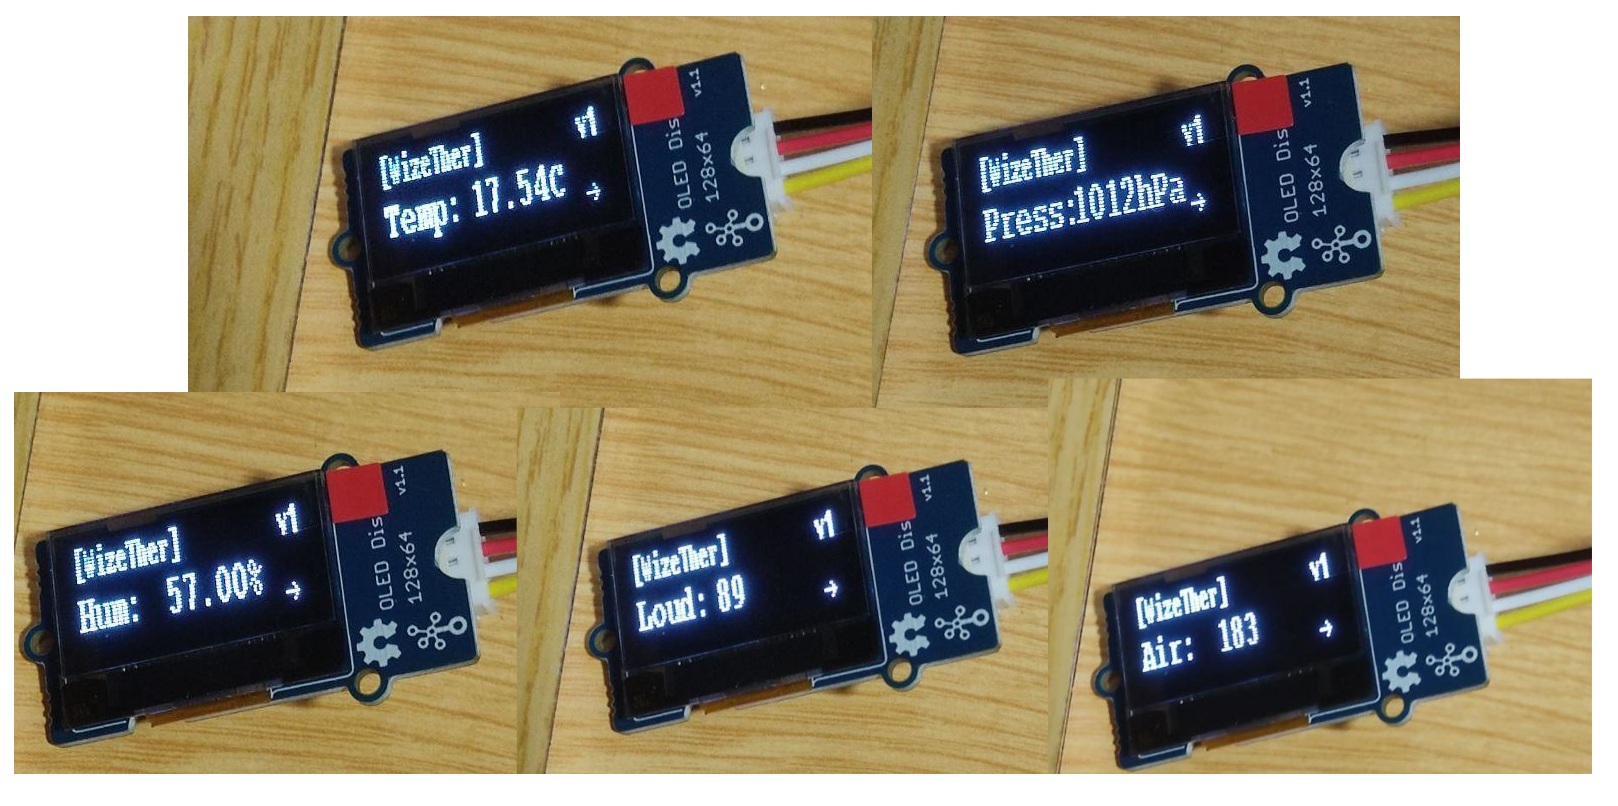
\includegraphics[width=0.65\textwidth]{img/Display_Wizether.png}
		\caption{Vistas de las diferentes pantallas \textit{Wizether}}
	\end{center}
\end{figure}


 \begin{figure}[h]
 	\begin{center}
 		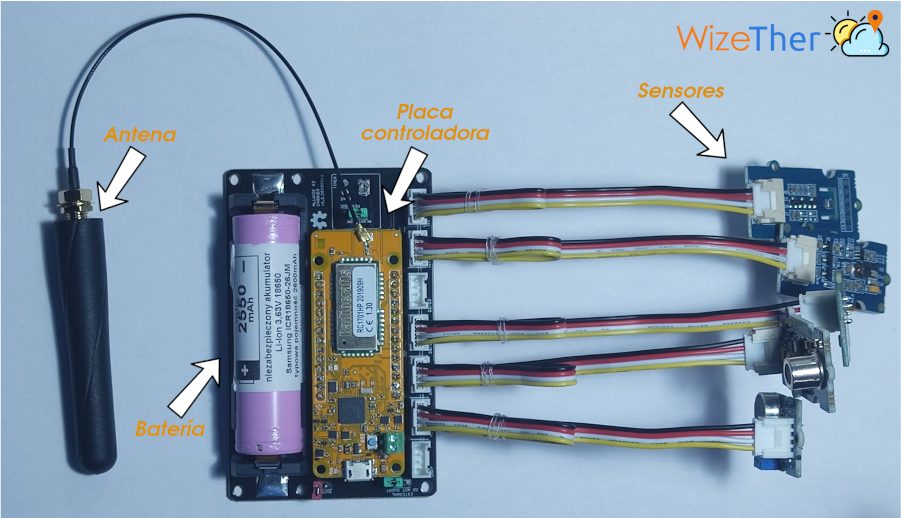
\includegraphics[width=0.75\textwidth]{img/info_wize_sensor_v1.png}
 		\caption{Infografía de una estación \textit{Wizether} (versión 1)}
 	\end{center}
 \end{figure}

\pagebreak

\noindent A medio y largo plazo, se requiriría de un despliegue de una red más amplia de estaciones \textit{WizeTher}, y por consecuente de gateways \textit{Wize}, para crear una red \textit{Wize} en la ciudad de Cartagena. De esta manera, el volumen de datos será mayor y más significativo, de cara a la toma de decisiones. \\

\begin{figure}[h]
	\begin{center}
		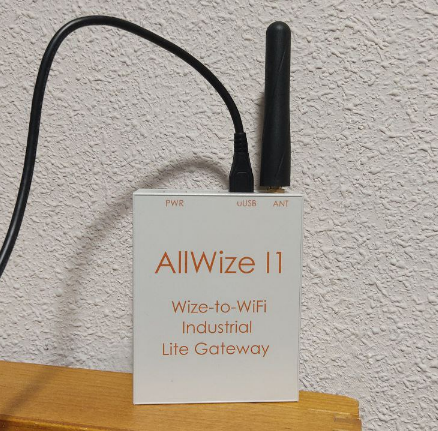
\includegraphics[width=0.45\textwidth]{img/gateway_wize.png}
		\caption{Fotografía de un gateway \textit{Wize}}
	\end{center}
\end{figure}

\noindent Cabe anotar que este elemento (ajeno a la estación pero necesario para la creación una red) ejerce la función de recibir los mensajes de una estación y subirlos a la nube a través de MQTT. Además, cada 5 minutos envía un mensaje MQTT al servidor indicando que el gateway sigue activo (detectando así posibles caídas del servicio desde el otro extremo). \\

\pagebreak

\subsection{Plataforma web}
Pensamos que para una mejor integración de la solución era necesaria la creación de una plataforma web, a la cual podemos acceder a través de \href{https://wizether.ranii.pro/}{\textit{Página web con acceso a plataforma web de \textit{WizeTher}}}. \\

\begin{figure}[h]
	\begin{center}
		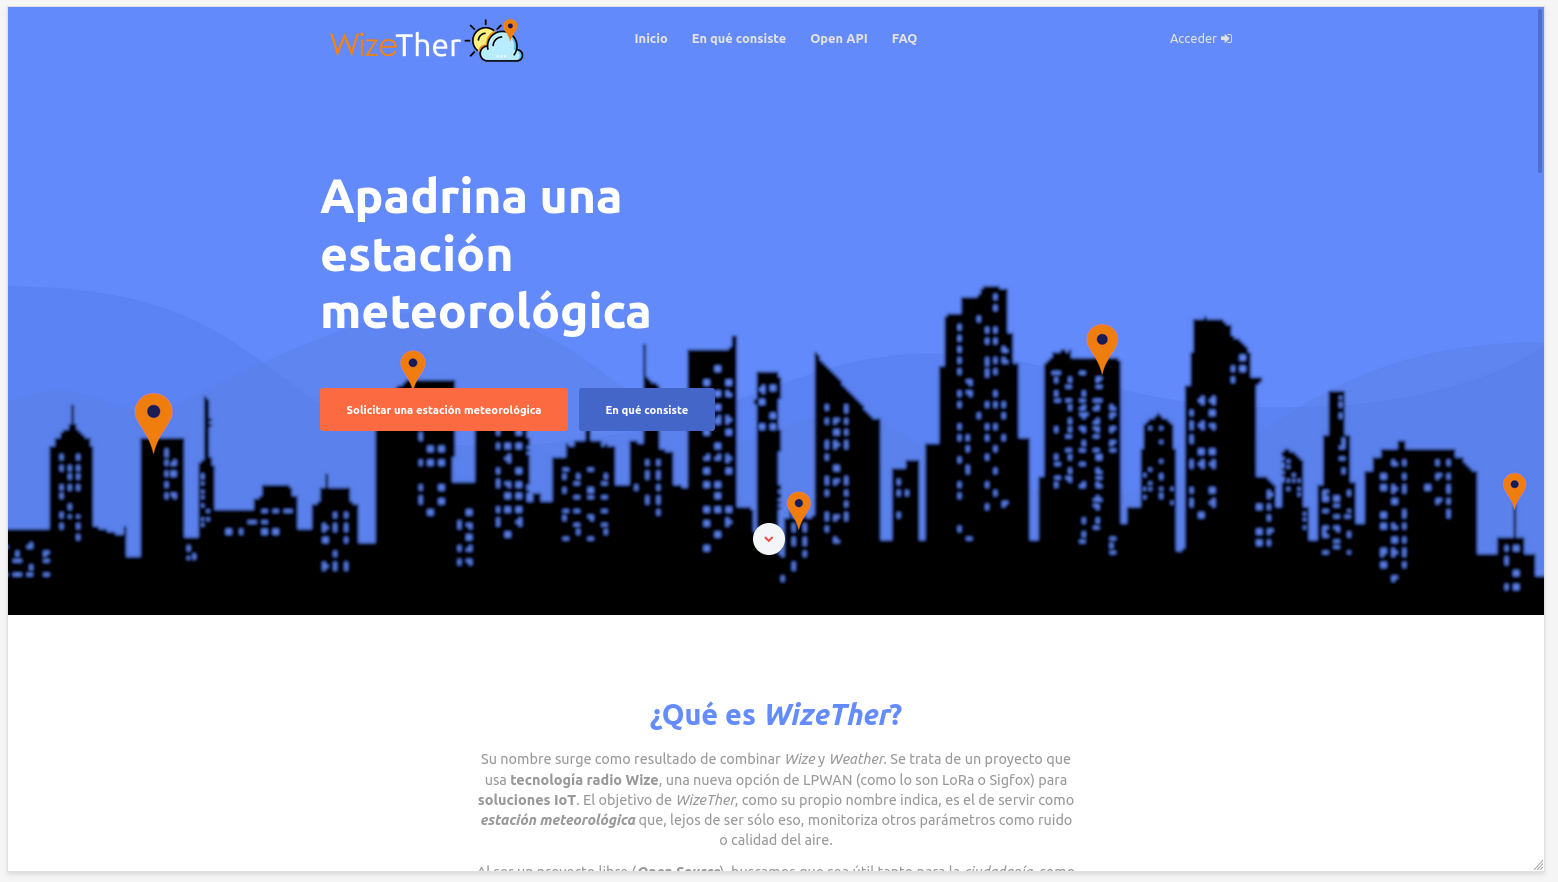
\includegraphics[width=0.7\textwidth]{img_rani/web_home.png}
		\caption{Captura web \textit{WizeTher} (inicio)}
	\end{center}
\end{figure}

\begin{figure}[h]
	\begin{center}
		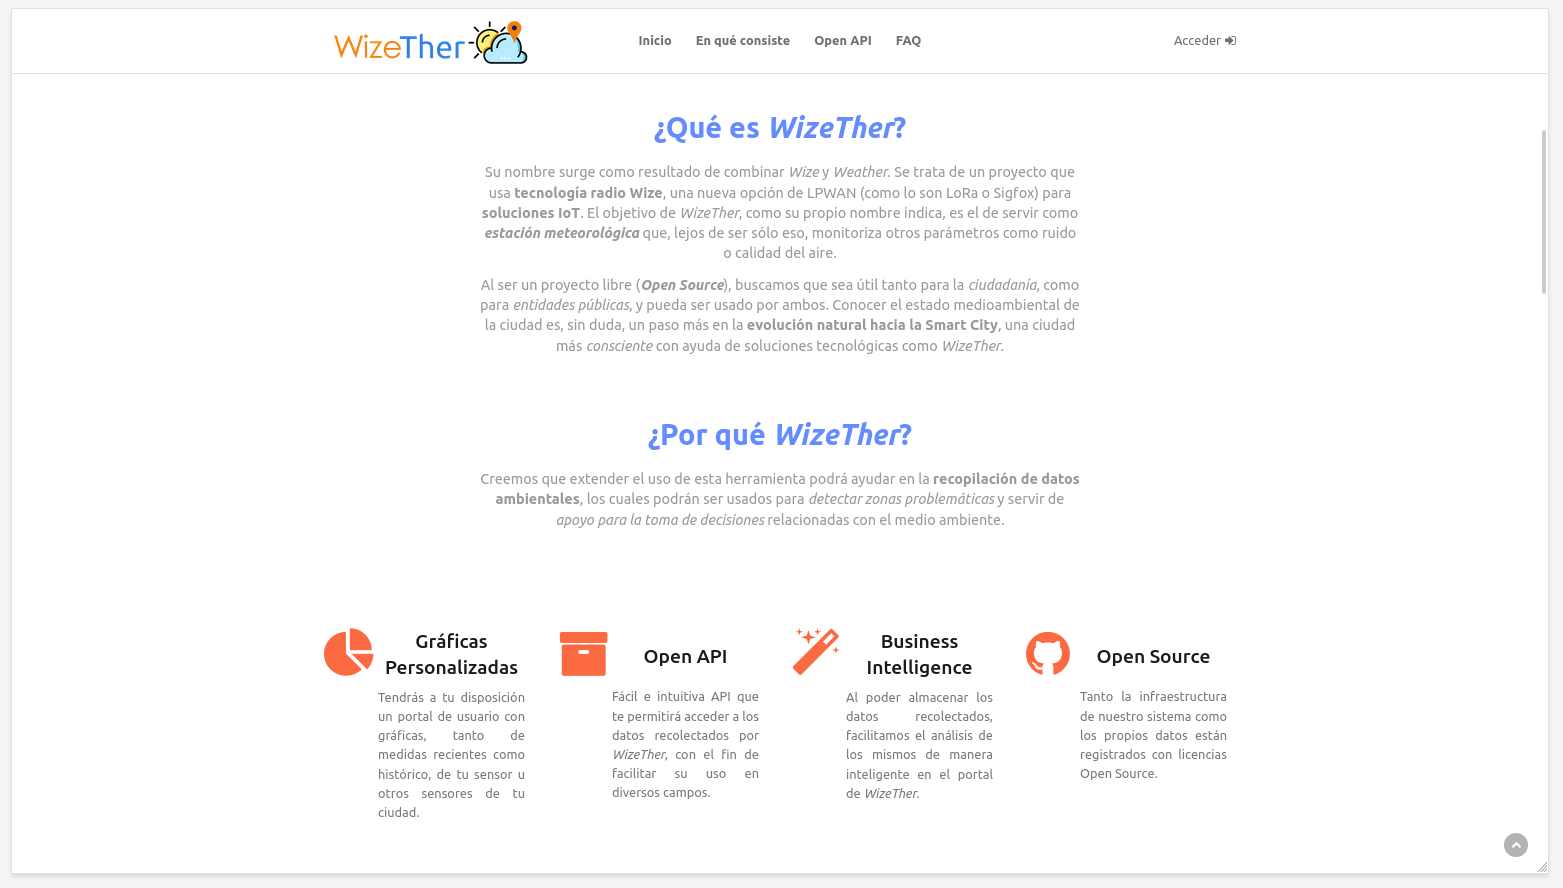
\includegraphics[width=0.7\textwidth]{img_rani/web_wizether.png}
		\caption{Captura web \textit{WizeTher} (Sobre \textit{WizeTher})}
	\end{center}
\end{figure}

\pagebreak

\subsubsection{Acceso a la plataforma web}

\noindent Se ha habilitado el acceso a la plataforma a través de un usuario de prueba (clicando sobre \textit{Acceder} en la esquina superior derecha de la página web):

\begin{itemize}
	\item Usuario: wizether@ranii.pro 
	\item Contraseña: wizether2021
\end{itemize}

\noindent Por motivos de seguridad, se ha deshabilitado temporalmente el registro de usuarios (sólo los administradores de la plataforma pueden crear nuevos usuarios).

\begin{figure}[h]
	\begin{center}
		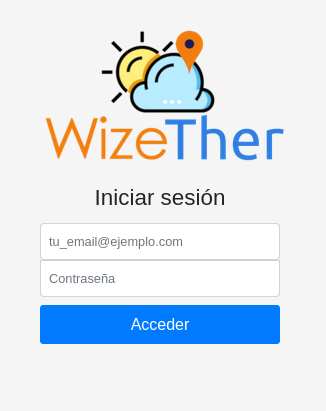
\includegraphics[width=0.25\textwidth]{img_rani/inicar_sesion.png}
		\caption{Captura inicio sesión en \textit{WizeTher}}
	\end{center}
\end{figure}

\begin{figure}[h]
	\begin{center}
		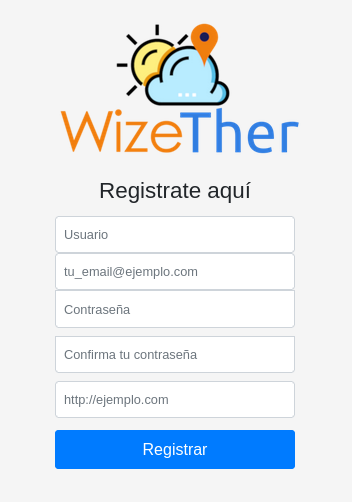
\includegraphics[width=0.25\textwidth]{img_rani/registro.png}
		\caption{Captura registro de nuevo usuario en \textit{WizeTher}}
	\end{center}
\end{figure}

\pagebreak

\subsubsection{Funcionalidades de la plataforma web}

Lo primero que aparece al iniciar sesión en la plataforma son una serie de gráficas donde se pueden visualizar datos recogidos por sensores de estaciones \textit{WizeTher} durante las últimas 24 horas. Además, se irán actualizando conforme el servidor vaya recibiendo datos nuevos. 

\begin{figure}[h]
	\begin{center}
		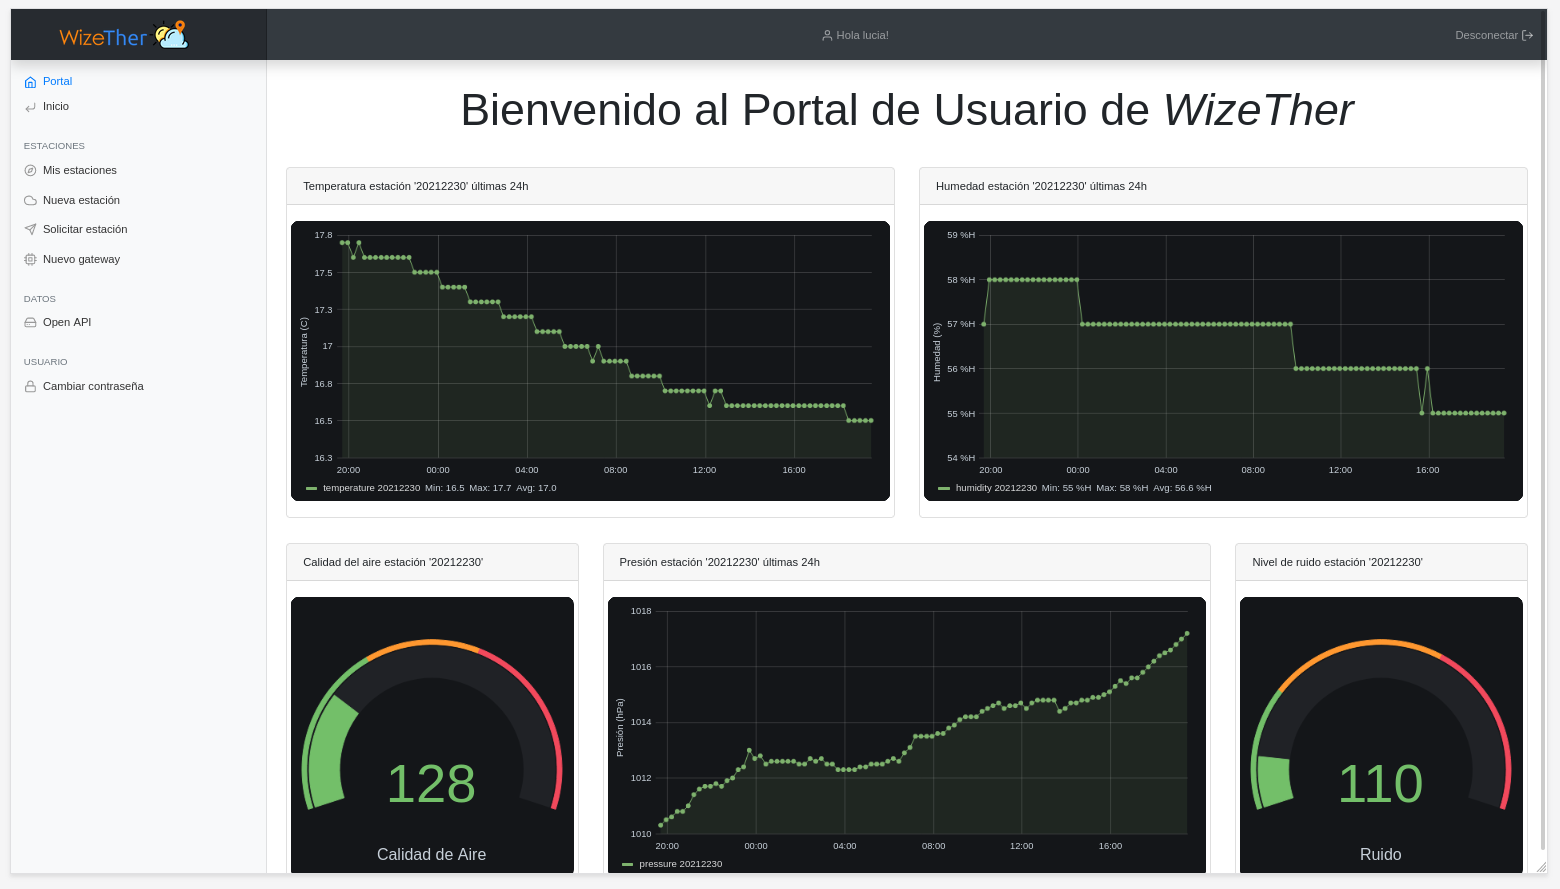
\includegraphics[width=0.8\textwidth]{img_rani/dashboard_user.png}
		\caption{Captura bienvenida portal en \textit{WizeTher}}
	\end{center}
\end{figure}

\pagebreak

\noindent En este apartado aparecerán las diferentes estaciones que se hayan dado de alta en el servidor, junto con su ubicación (longitud, latitud e interior/exterior) y su estado (apagada, activa o durmiendo).

\begin{figure}[h]
	\begin{center}
		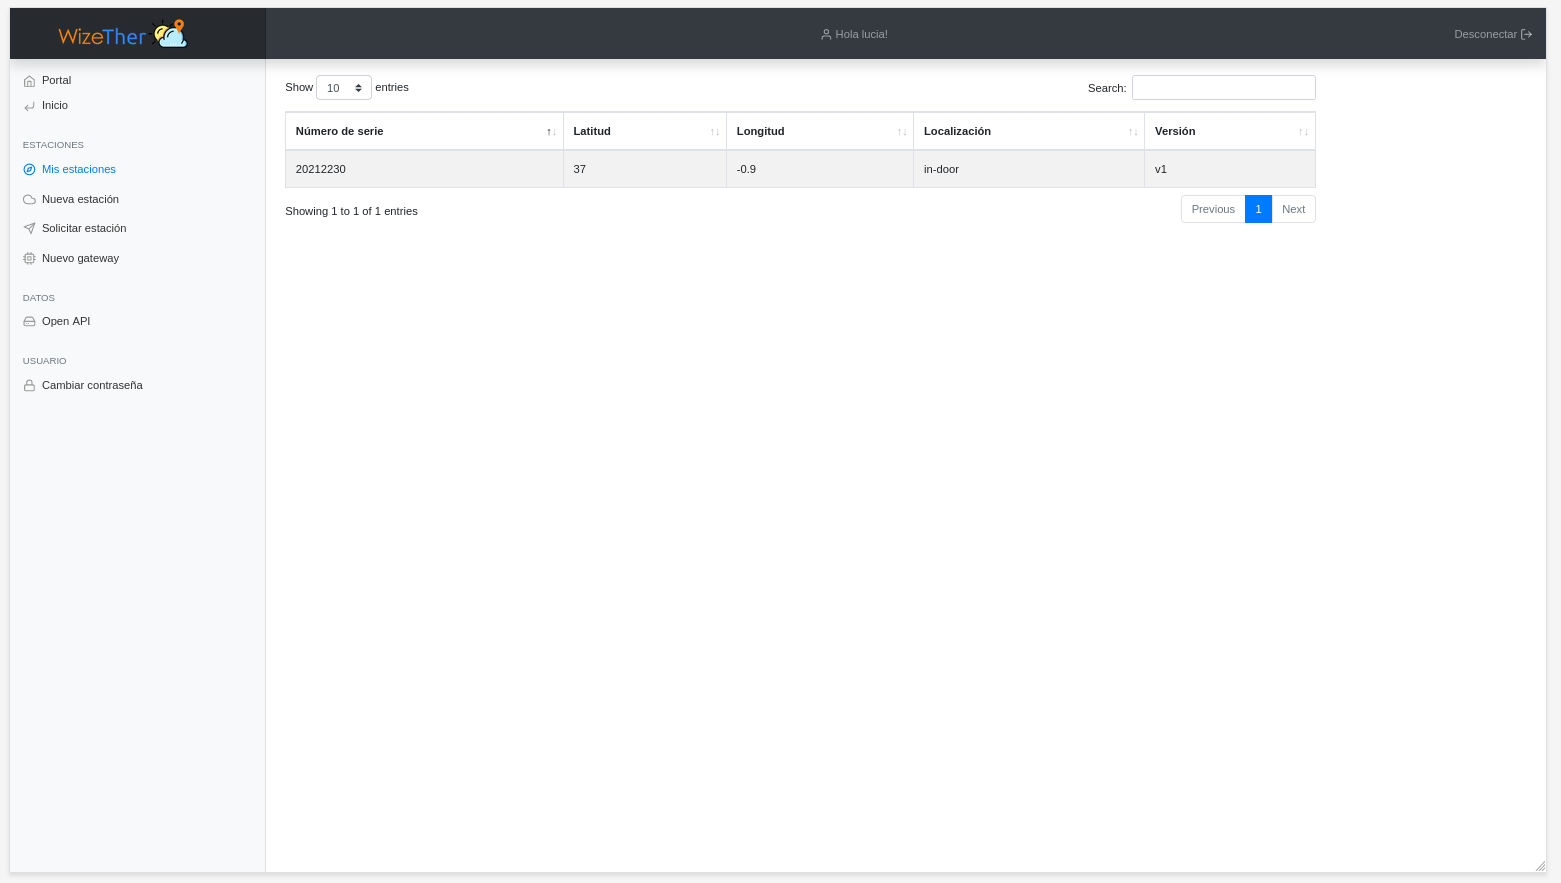
\includegraphics[width=0.8\textwidth]{img_rani/mis_estaciones.png}
		\caption{Captura \textit{Mis estaciones} en \textit{WizeTher}}
	\end{center}
\end{figure}

\pagebreak

\noindent En el apartado \textit{Nueva estación} podemos dar de alta una estación en el servidor, introduciendo los datos \textit{Número de serie}, \textit{Longitud} y \textit{Latitud}, pudiéndonos ayudar para ubicar la estación del mapa que aparece a la derecha (haciendo clic sobre él, se autocompletan los datos de \textit{Longitud} y \textit{Latitud}). Además, se requiere seleccionar dónde está ubicada la estación, en interior o exterior.

\begin{figure}[h]
	\begin{center}
		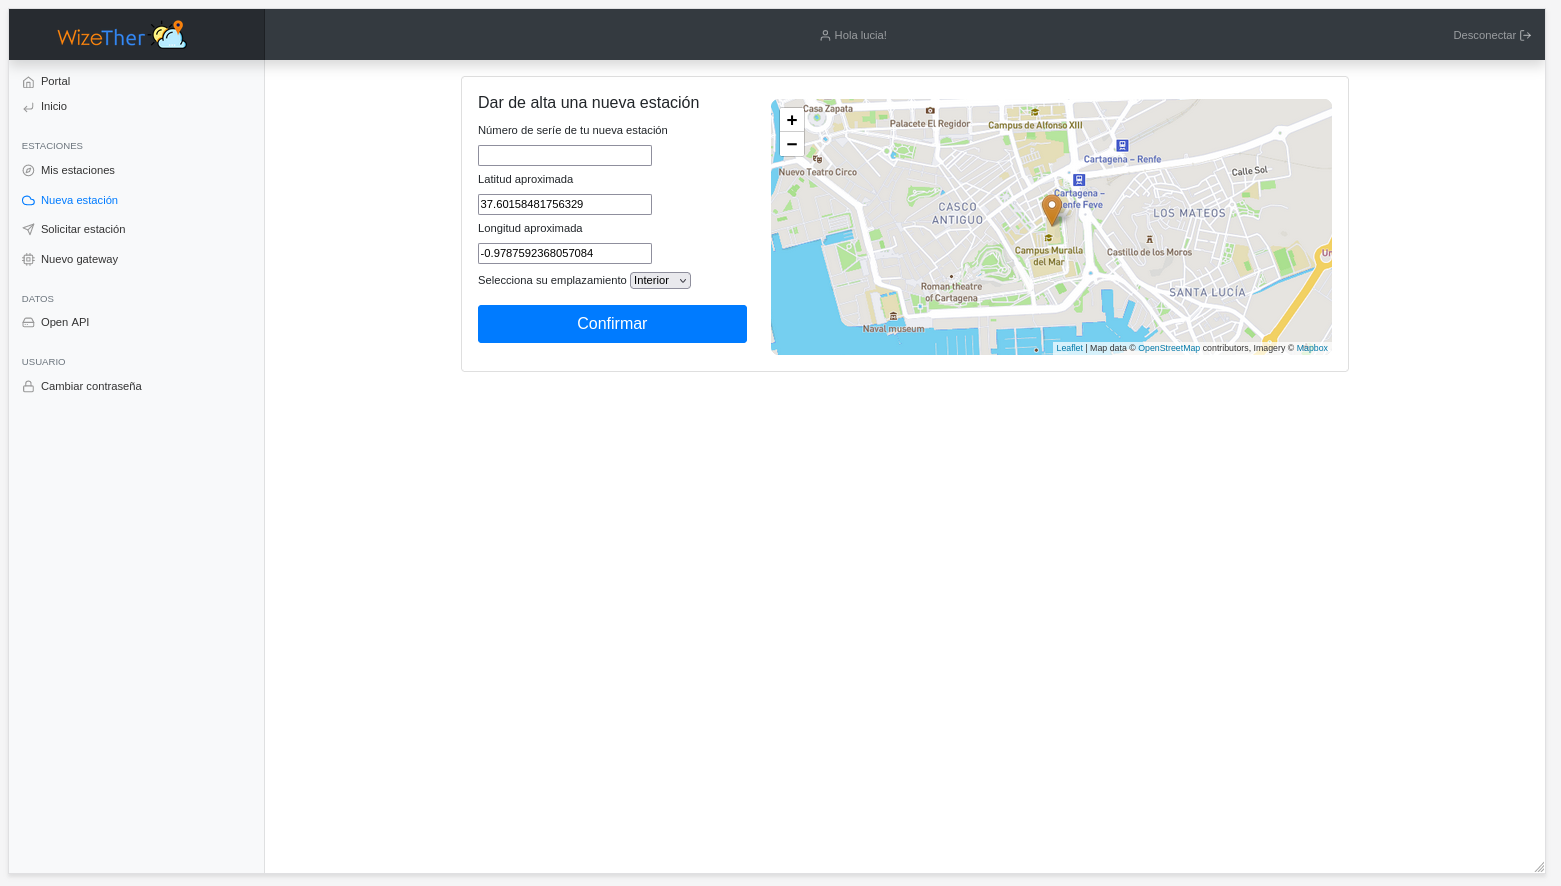
\includegraphics[width=0.8\textwidth]{img_rani/nueva_estacion.png}
		\caption{Captura \textit{Nueva estación} portal en \textit{WizeTher}}
	\end{center}
\end{figure}

\pagebreak

\noindent

\noindent En el apartado \textit{Nuevo gateway} podemos añadir un nuevo gateway completando los mismos parámetros que en el apartado \textit{Nueva estación}, y además nos encontramos con un nuevo campo (\textit{Potencia de transmisión}) que nos permite modificar el alcance visual de nuestro gateway  (se observa en el mapa).

\begin{figure}[h]
	\begin{center}
		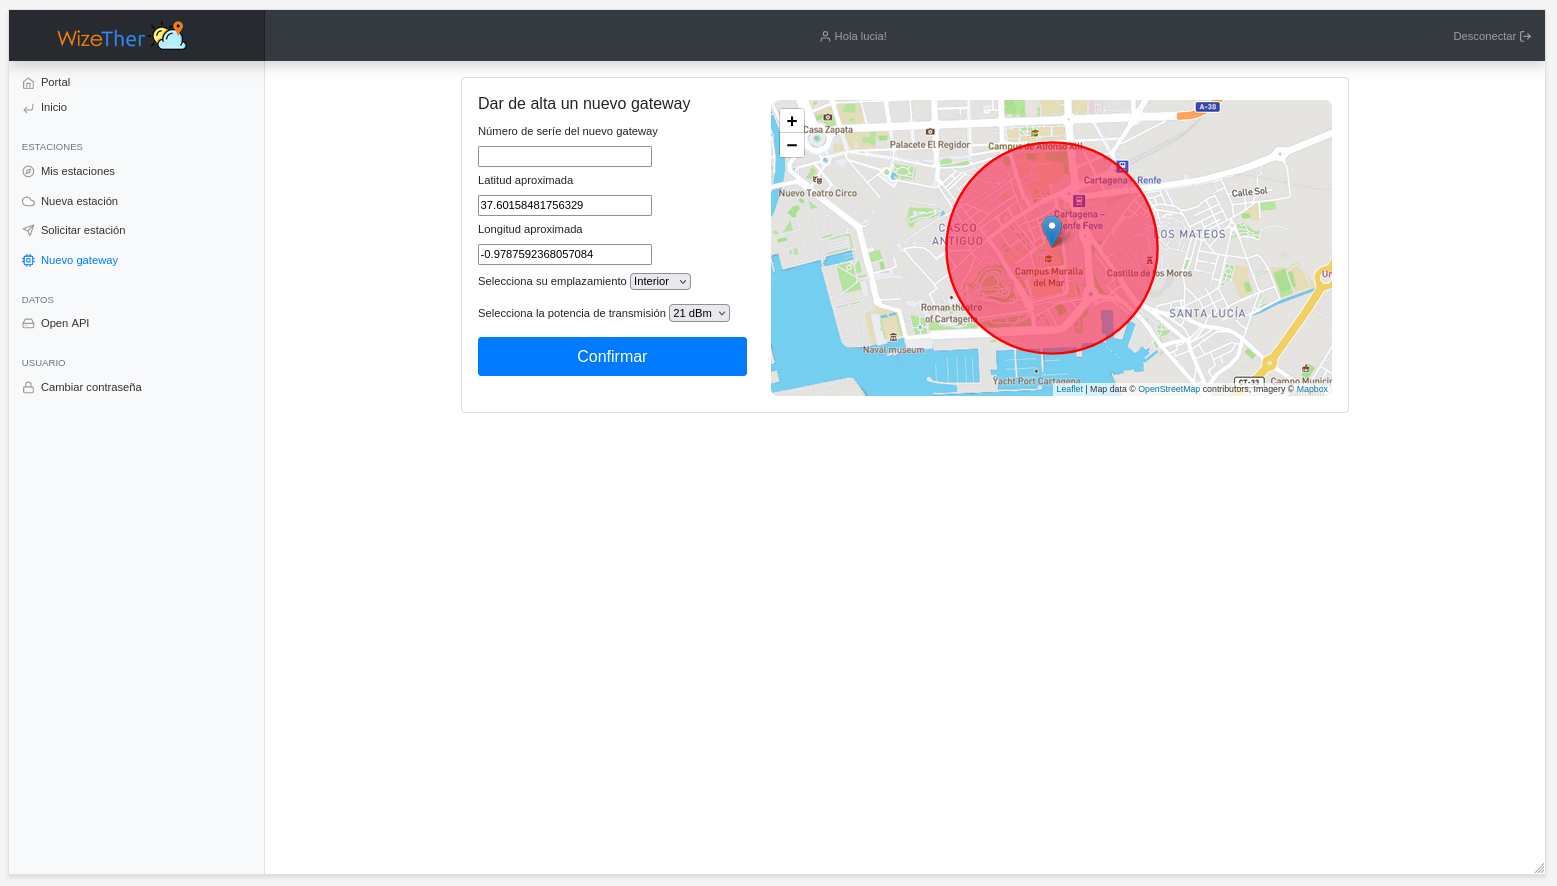
\includegraphics[width=0.8\textwidth]{img_rani/nuevo_gateway.png}
		\caption{Captura \textit{Nuevo gateway} portal en \textit{WizeTher}}
	\end{center}
\end{figure}

\pagebreak

\subsection{Open API}
Como funcionalidad extra que vimos necesaria para complementar el estudio medioambiental, está la \textit{Open API}. Una API es una interfaz de programación que nos permite facilitar el acceso a la información de nuestra base de datos; en este caso, la salida de la API es en formato CSV. A través de ella podemos realizar una serie de consultas que nos devuelven los datos relacionados que nos encontremos en la base de datos.

\begin{figure}[h]
	\begin{center}
		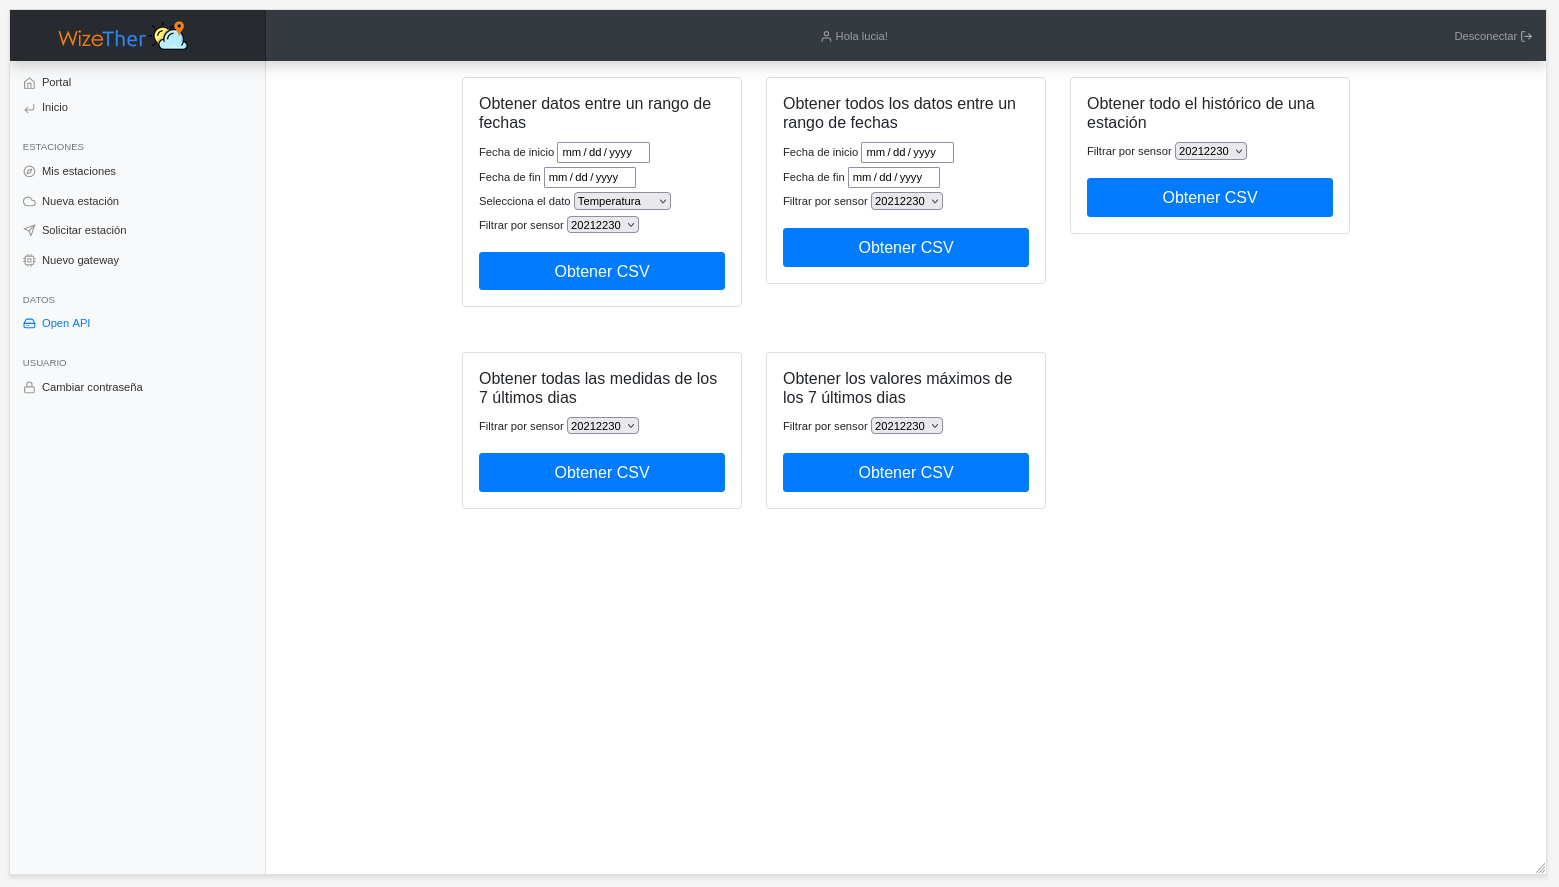
\includegraphics[width=0.8\textwidth]{img_rani/open_api.png}
		\caption{Captura \textit{Open API}  en \textit{WizeTher}}
	\end{center}
\end{figure}


\noindent Por último, anotar que el nombre de \textit{Open API} viene de una de las funcionalidades  propias de \textit{WizeTher}, que es la de permitir a los usuarios acceder a los datos de las estaciones registradas en el servidor; además, también recuerda a \textit{Open Source}, una característica del proyecto, el ser ofrecido bajo esa filosofía, por lo que los datos que se descargan a través de la API son \textit{open}.

\pagebreak

\section{Resumen}

\section{Fuentes complementarias}

\pagebreak

\section{Anexo. Detalle técnico sobre infraestructura \textit{Wizether}.}

\noindent Actualmente, la infraestructura que da soporte al ecosistema \textit{Wizether}, esta compuesta por tres partes. 

\begin{enumerate}
	\item La primera parte corresponde con la captación de datos, dichos datos son detectados por las estaciones, las cuales los transmitirán a los gateway utilizando la tecnología radio \textit{Wize}. Una vez los datos han llegado al gateway, son encapsulados en un mensaje MQTT (tipo publish) que se subirán a un topic específico en el servidor destino.
	
	\item En la segunda parte del sistema, correspondiente con el procesado de los datos en el servidor. Nuestro broker de MQTT, mosquitto, recepciona los paquetes MQTT entrantes y actualiza a todos los clientes que previamente se han suscrito a estos topics. En nuestro caso, utilizamos NodeRed para transformar los mensajes MQTT en datos aptos para guardarlos en una base de datos de tipo Time Series, en este caso, InfluxDB (en su versión 2.0, incluyendo ventajas como son el lenguaje Flux).
	
	\item La tercera parte de nuestro sistema, corresponde con la representación de los datos. En este apartado encontramos la aplicación Grafana, encargada de representar los datos que tenemos almacenados en InfluxDB. Por otro lado, encontramos \textit{Wizether\_webapp}, que tiene por función aportar la lógica característica a lo que sería \textit{Wizether} (OpenAPI, portal de usuarios, registro de estaciones...)
\end{enumerate}

\noindent A modo resumen, un esquemático de la infraestructura que estamos utilizando, podría ser el siguiente:

\begin{figure}[h]
	\begin{center}
		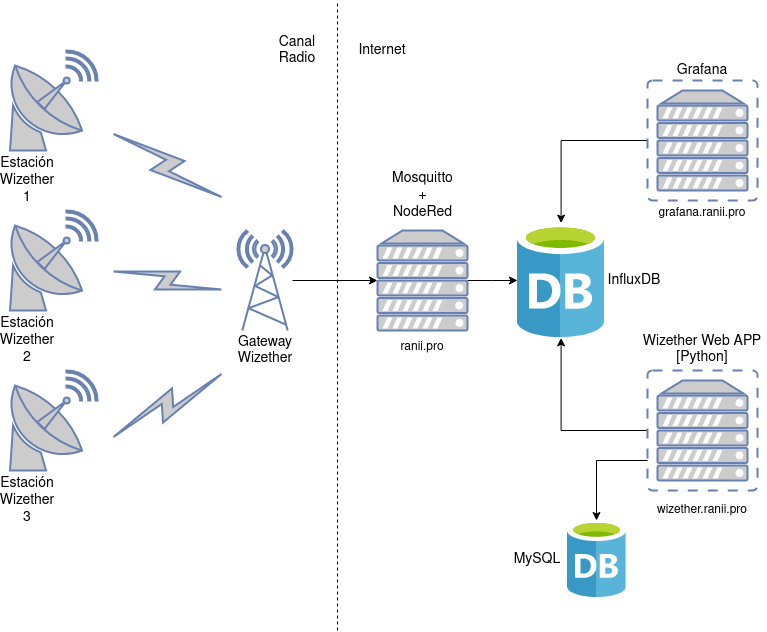
\includegraphics[width=0.6\textwidth]{img_rani/WizeTher_infraestructura.png}
		\caption{Esquema infraestructura \textit{Wizether}}
	\end{center}
\end{figure}

\pagebreak

\subsection{Servidor ranii.pro}
\noindent Utilizamos un servidor dedicado para hacer de host de nuestros servicios. Para levantar cada una de las diferentes aplicaciones, hemos utilizado \textit{Docker}, con ayuda del asistente \textit{docker-compose}. Además, como proxy de entrada HTTP, nos hemos favorecido de \href{https://traefik.io/}{Traefik} (versión 2.0), facilitándonos la creación de subdominios específicos para los contenedores y aportando los certificados necesarios para establecer comunicaciones seguras entre ellos. Hemos desplegado los siguientes subdominios:
\begin{itemize}
	\item \href{https://nodered.wize.ranii.pro}{https://nodered.wize.ranii.pro} 
	
	\item \href{https://grafana.wize.ranii.pro}{https://grafana.wize.ranii.pro} 
	
	\item \href{https://influxdb.wize.ranii.pro}{https://influxdb.wize.ranii.pro} 
	
	\item \href{https://wizether.ranii.pro}{https://wizether.ranii.pro} 
	
\end{itemize}

\noindent Además, de manera complementaria, se ha utilizado la plataforma de integración continua \href{https://www.drone.io/}{Drone.CI} para desplegar de manera rápida y segura los servicios de \textit{Wizether\_webapp}. Esta aplicación se encuentra alojada en: \href{https://drone.ranii.pro}{https://drone.ranii.pro}. \\

\noindent \textit{Disclaimer}. Muchas de las páginas referenciadas en este anexo, por no decir la mayoría,  tienen un login asociado. Sin embargo, creemos que es importante mencionarlas ya que sin ellas no habría sido posible el desarrollo de \textit{Wizether}.

\subsection{Aplicación web Wizether.}
\noindent Para la plataforma web de \href{https://wizether.ranii.pro/}{\textit{Wizether}}, hemos utilizado como lenguaje de programación Python complementándolo con el framework de desarrollo web \href{https://flask.palletsprojects.com/en/1.1.x/}{Flask}. Algunas de las características importantes que dispone nuestro sistema son las siguientes:
\begin{itemize}
	\item Página de bienvenida.
	\item Portal de usuarios.
	\item Portal de administración.
	\item Sistema de acceso, registro y cambio de contraseña.
	\item Base de datos dedicada (MySQL).
	\item Formulario protegidos contra CSRF.
	\item Tareas asíncronas utilizando redis.
	\item Control de acceso dependiendo del rol del usuario.
	\item Conexión a InfluxDB. Consultas utilizando el lenguaje Flux.
	\item Descarga de datos tipo Time Series en formato CSV.
	\item Acceso e interacción con mapas geográficos.
\end{itemize}

\noindent Todo el código de la aplicación esta público en el repositorio de GitHub: \href{https://github.com/Raniita/wizether_webapp}{Wizether\_webapp}.\\

\end{document}

%https://46eybw2v1nh52oe80d3bi91u-wpengine.netdna-ssl.com/wp-content/uploads/2016/03/Internet-of-Things-2016.png